\chapter{Introducción}

Este trabajo Fin de Grado se centra en dos temas: por un lado el tratamiento digital de imagen (TDI) como una rama de conocimiento que se está empleando en el desarrollo de muchas investigaciones en diferentes campos, y por otro la docencia y lo importante que es que ésta sea accesible a todo el que esté interesado en aprender sobre un tema nuevo.\\ 

El trabajo consiste en la creación de un entorno de prácticas basado en cuadernillos Python para la asignatura de TDI de los grados ETSIT-URJC con el objetivo de hacerlas más accesibles, tanto a alumnos que cursan la asignatura, como a alumnos externos a la ETSIT.\\



\section{Tratamiento de imagen}

El tratamiento de la imagen pertenece a la rama de Visión Artificial que es una disciplina científica que trata de adquirir, procesar y analizar imágenes con el fin de extraer una serie de características que puedan ser utilizadas por un ordenador para comprender esa imagen.\\

La disciplina del tratamiento de imagen trata de la extracción de información de una o varias imágenes usando métodos matemáticos que tratan la imagen como una señal o matriz. Estos métodos pueden centrarse en mejorar la calidad de la imagen, añadir efectos o facilitar la búsqueda de información. El Tratamiento Digital de Imagen usa ordenadores para aplicar estas transformaciones donde una imagen digital está compuesta de un número finito de elementos, cada uno con posición y valor particular (píxel)\cite{Historia2}.\\

Una de las razones principales que hacen que este campo sea tan complejo es la diferencia en cómo vemos imágenes nosotros y cómo las ``ve'' un ordenador. Nuestro cerebro analiza imágenes siempre en un contexto y con referencias para comparar, mientras que un ordenador recibe una serie de datos finitos en los que se ha perdido por el camino mucha información, por ejemplo si el objeto de la imagen es tridimensional, de dónde viene la imagen y el contexto de esa imagen. Esto hace que cosas que para la vista humana son obvias, para un ordenador sean operaciones muy complejas que requieran múltiples transformaciones y algoritmos para extraer ciertas características que se puedan contrastar con una base de datos.\\

El tratamiento de imagen se puede dividir en tres procesos diferentes que se pueden dar secuencialmente en el análisis de una imagen o a la vez. Estos procesos son: pre-procesado, segmentación y análisis. La asignatura de TDI se centra sobre todo en métodos de pre-procesado y segmentación de imágenes.\\ 

Un elemento que ha precipitado el crecimiento y la necesidad del tratamiento digital de imagen es el crecimiento en el uso y calidad de las cámaras digitales. Antes del uso común de estas cámaras la única manera de conseguir una imagen digital era digitalizando una fotografía realizada e impresa con una cámara analógica. Este es  un proceso que conlleva bastantes problemas ya que puede contaminar la imagen con ruido, además de ser un proceso tedioso, lo que limitaba la cantidad de imágenes disponibles para usar en tratamiento de imagen. También se podían conseguir imágenes digitales con aparatos muy especializados como pueden ser aparatos usados en el campo de la medicina.\\

La primera cámara digital se inventó en 1975. Una vez se comercializó aumentó la cantidad de imágenes que se pueden usar para el tratamiento de imagen. La mejora de la calidad de imagen que producen las cámaras digitales es importante ya que ahorran pasos de preprocesado si no se tiene que limpiar la imagen de ruido. Las cámaras personales no son la única fuente de imágenes digitales, también generan imágenes digitales los microscopios y telescopios electrónicos o las máquinas como la de resonancia magnética.\\


\subsection{Historia}
Uno de los primeros ejemplos de tratamiento de imágenes digitales se dio en la década de los años 20 cuando se empezaron a enviar imágenes a través de un cable submarino de Londres a Nueva York. El sistema de transmisión de imágenes por cable de Bartlane usaba un telégrafo (Figura \ref{telegrafo}) para transmitir imágenes por el Atlántico\cite{Historia3}. Inicialmente estas imágenes tenían 5 niveles de gris, pero fue ampliado a 15 niveles en 1929. Estas imágenes son consideradas las primeras imágenes digitales. La Figura \ref{1digital} muestra una imagen transmitida usando este sistema. Ya desde esta época se pudo ver que el principal problema que surgía con la imagen digital es la cantidad de espacio y capacidad computacional que requieren.\\

\begin{figure}[h]
\centering
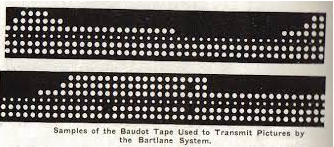
\includegraphics[width=0.6\textwidth]{imagenes/telegrafo}
\caption{Tira de Baudot.}
\label{telegrafo}
\end{figure}

\begin{figure}[h]
\centering
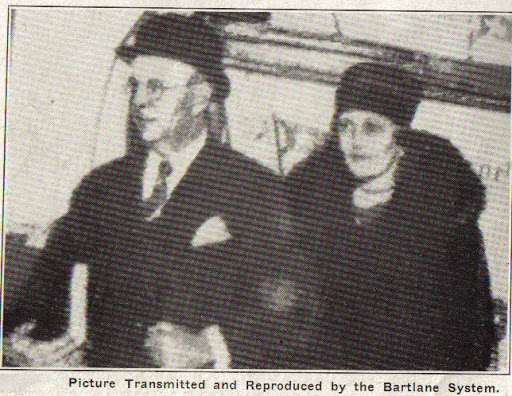
\includegraphics[width=0.6\textwidth]{imagenes/1digital}
\caption{Imagen transmitida usando el sistema de Bartlane.}
\label{1digital}
\end{figure}

Los avances en este campo en los primeros años dependían completamente del avance de los ordenadores y su capacidad tanto de almacenamiento como computacional.\\

Los primeros avances en el tratamiento digital de imágenes se dieron en los años 70 en el campo de la medicina y en astronomía. En medicina lo que impulsó esta necesidad para analizar imágenes digitales fue la invención del TAC (tomografía axial computarizada) que consiste en una serie de algoritmos que toman varias fotografías realizadas con rayos x para construir una imagen tridimensional. Se usan varias operaciones de tratamiento de imagen para mejorar el contraste de la imagen o pasar los diferentes niveles de gris a color para facilitar la interpretación.\\



\subsection{Aplicaciones}
El tratamiento digital de imagen tiene aplicaciones en una amplia variedad de campos desde medicina a diseño, pasando por astronomía y robótica\cite{Usos}.  Estos son algunos ejemplos de campos en los que se usan herramientas de tratamiento de imagen:
\begin{itemize}
\item \textbf{Medicina y biología}: El tratamiento de imágenes digital se usa para una gran cantidad de análisis. Un ejemplo son las imágenes médicas, en el proceso de crear una representación visual de la estructura interior de un cuerpo antes de una intervención. También crea una representación visual de cómo funcionan varios órganos o tejidos. Esto se consigue gracias a varios avances en métodos como las tomografías computarizadas o las resonancias magnéticas.\\

Por ejemplo ahora se está usando en la detección de tumores\cite{Tumores}. Para esto se usan imágenes obtenidas con resonancia magnética y métodos de aprendizaje máquina que permiten comparar miles de imágenes para clasificar tumores. Para que las imágenes puedan ser usadas por el algoritmo de aprendizaje tienen que ser procesadas y se tienen que extraer características de interés, para esto se usan varios métodos de tratamiento de imagen estudiados en la asignatura como la segmentación de objetos, esto se puede ver en la Figura \ref{tumores}.\\

\begin{figure}[h]
\centering
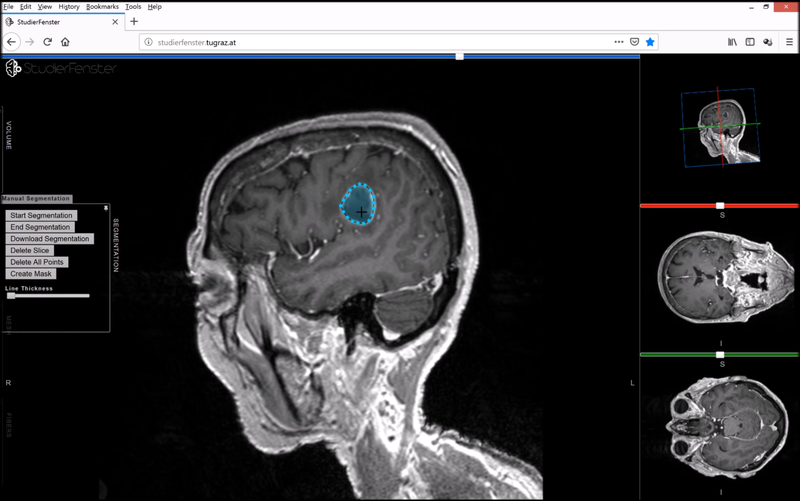
\includegraphics[width=0.8\textwidth]{imagenes/tumores.png}
\caption{Segmentación de un tumor cerebral.}
\label{tumores}
\end{figure}

Dentro del campo de la biología el tratamiento de imagen se está empleando para analizar imágenes sacadas de microscopio, por ejemplo para automatizar el cómputo de células en una imagen.\\

\item \textbf{Robótica}: En este campo se utilizan herramientas de tratamiento digital de imagen para intentar emular la visión humana. Su objetivo es reconocer objetos e información relevante de una forma similar a como lo hacemos los humanos. Se está aplicando en el campo de la robótica para la conducción automática de coches o brazos automatizados.\\

Por ejemplo se aplica en casos de control basado en visión, que consiste en el uso de información obtenida a través de una cámara para calcular el movimiento de un robot\cite{vision}. Se puede estimar la posición del robot usando la reconstrucción 3D de un espacio a partir del análisis de imágenes 2D de ese espacio. Un método para conseguir este espacio 3D es \emph{stereovision} que consiste en extraer un mismo objeto de varias imágenes (Figura \ref{stereovision}) y triangular su posición, para esto se necesitan al menos dos cámaras\cite{stereovision}.

\begin{figure}[h]
\centering
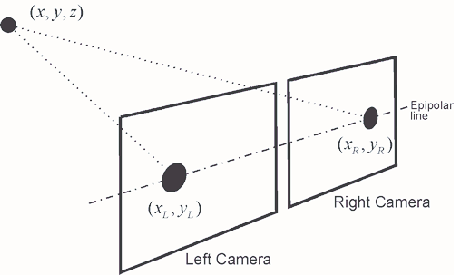
\includegraphics[width=0.8\textwidth]{imagenes/stereovision.png}
\caption{Esquema que demuestra el funcionamiento de \emph{stereovision}}
\label{stereovision}
\end{figure}

\item \textbf{Restauración}: Otro campo en el que se usan las herramientas de tratamiento de imágenes es la reparación de imágenes (Figura \ref{restauracion}) o videos dañados, ya sea por antigüedad o cualquier otra causa. \\

\begin{figure}[h]
\centering
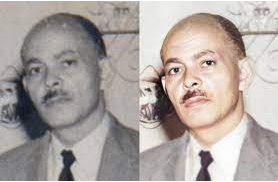
\includegraphics[width=0.8\textwidth]{imagenes/restauracion}
\caption{Imagen restaurada y coloreada usando tratamiento de imagen.}
\label{restauracion}
\end{figure}

\item \textbf{Geografía}: El tratamiento de imagen también se usa para crear mapas analizando imágenes de satélite y otros muchos análisis del terreno. Por ejemplo en agricultura Artizzu et al.\footnote{X. P. B. Artizzu, A. Ribeiro, A. Tellaeche, G.Pajares, C. F. Quintanilla (2009), Improving weed pressure assessment using digital images from an exp, ya que además de usar re, 65, pp. 176–185,
2009} diseñó un sistema que analiza imágenes del suelo y utiliza el color y la textura de la imagen para averiguar qué está plantado en esa zona.\\

El mejor ejemplo de este uso es Google Maps, ya que además de usar información de bases de datos de mapas previos, usa imágenes de satélite para cuadrar y corregir rutas y las imágenes de ``\emph{street view}'' para detección de señales, por ejemplo las de velocidad que luego usa en su función de planificación de rutas\cite{maps}.

\item \textbf{Seguridad}: Un tema por el que el tratamiento de imagen está recientemente en la noticias es su uso en seguridad, específicamente por la identificación facial en cámaras de seguridad. También se emplea en otras verificaciones biométricas, por ejemplo las huellas dactilares.\\

Otro ámbito de la seguridad en el que se usa el tratamiento de imagen es en la estenografía y la encriptación, por ejemplo para crear firmas digitales irremovibles en obras de arte o documentos (Figura \ref{estenografia}).\\

\begin{figure}[h]
\centering
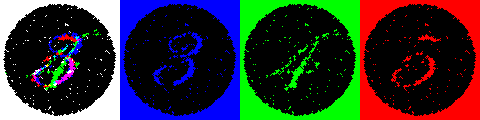
\includegraphics[width=0.8\textwidth]{imagenes/Steganography.png}
\caption{Ejemplo básico de estenografía.}
\label{estenografia}
\end{figure}
\item \textbf{Transmisión y codificación}: Herramientas de tratamiento de imagen como el análisis de imágenes en frecuencia o  la reducción de niveles se usan a menudo para la codificación de imágenes y videos con el objetivo de que ocupen menos espacio y facilitar su transmisión. Por ejemplo en el tema de video de la asignatura se estudian métodos de predicción de fotogramas usados de manera habitual para codificar videos.\\

\item \textbf{Diseño y edición gráfica}: Seguramente el uso más común del tratamiento de imagen es el diseño. Cualquier programa de uso común, como puede ser Photoshop, lo que tiene detrás de su interfaz son herramientas de tratamiento como filtros Gaussianos o filtros de detección de ejes.\\

\item \textbf{Teléfonos móviles}: En nuestra vida diaria también usamos herramientas de tratamiento de imagen a través del teléfono móvil, por ejemplo en el auto-enfoque de la cámara programado para detectar caras o en la lectura de códigos QR, que cada vez se usa más para validar unas entradas, como enlaces a cartas en restaurantes o en billetes de avión. Para los códigos QR la cámara del teléfono tiene que reconocer la imagen como un código QR, hacer varias transformaciones para colocarlo de forma digital y que se pueda analizar.\\

Un ejemplo muy claro del uso de tratamiento de imagen es Captio, una aplicación que usamos en el trabajo para subir las facturas del taxi. En esta aplicación subes una fotografía de una factura realizada con el teléfono y la aplicación extrae el texto de la factura, lo analiza y guarda la información con el objetivo de automatizar el sistema de gastos en nombre de la empresa. En la Figura \ref{taxi} se puede ver el tipo de información que extrae la aplicación de una factura de taxi.\\

\begin{figure}[h]
\centering
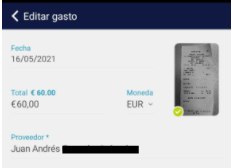
\includegraphics[width=0.6\textwidth]{imagenes/taxi.PNG}
\caption{Captura de pantalla de la aplicación Captio.}
\label{taxi}
\end{figure}

Esta no es la única aplicación que usa el tratamiento de imagen para leer texto, por ejemplo existen aplicaciones para ayudar a personas con problemas de visión que al hacer una fotografía a un texto lo leen en alto o aplicaciones que traducen textos por poner algunos ejemplos.\\

\end{itemize}

\section{Docencia de TDI}

Debido al rápido avance de las tecnologías nos encontramos en un campo que requiere una formación constante para mantenerse al día, siempre hay una nueva versión de algo que conocías con la que familiarizarte, nuevos avances o inventos revolucionarios. De ahí que exista todo un mundo de cursos de pago, o cursos ofrecidos por las empresas para informar a sus trabajadores de nuevos avances que se tienen que implementar para mantenerse a la vanguardia.\\

Desde la invención de internet la gente lo ha usado para aprender sobre todo tipo de temas\cite{KUO201435}. En los últimos años el número de personas autodidactas ha ido creciendo gracias a esta nueva herramienta global. Se usa para aprender sobre todo tipo de temas, desde manualidades hasta filología, pero debido a la complejidad de los temas técnicos como es el tratamiento de imagen puede resultar intimidante e inaccesible. Por eso es importante que se creen plataformas que faciliten el acceso a estos temas usando un lenguaje técnico pero sencillo y con enlaces a más recursos que permitan el acceso a la información necesaria para aprender sobre un tema nuevo, ya sea por necesidad o pura curiosidad.\\

En cuanto a formas de estudiar tratamiento de imagen en específico es una asignatura que se estudia en varias universidades, en diferentes carreras, normalmente relacionadas con imagen y video, ingeniería biomédica o robótica. También existe la posibilidad de acceder a cursos \emph{online} sobre este tema en sitios como Coursera que por ejemplo tiene un curso de procesamiento de imagen con Python o EDX que tiene algunos cursos de procesamiento de imagen orientado a diferentes campos como \emph{``Image Processing and Analysis for Life Scientists''}\footnote{\url{https://www.edx.org/course/image-processing-and-analysis-for-life-scientists?index=product&queryID=dbd34bf4ece2394643cfaff4d852d495&position=1}}. También existen videos en Youtube sobre este tema, con descripciones generales del campo, clases enteras dadas por expertos y subidas de forma gratuita, otro género común son los videos más específicos sobre aplicaciones concretas o programación (Figura \ref{youtube}).\\

\begin{figure}[h]
\centering
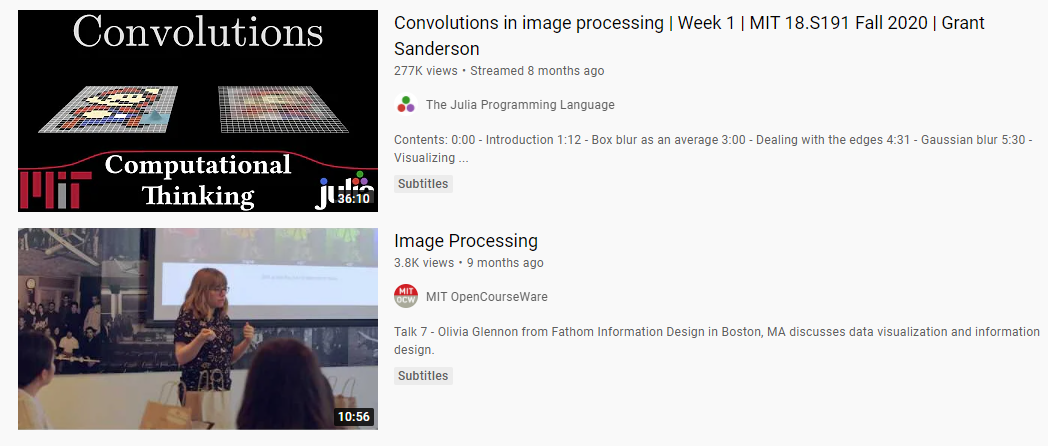
\includegraphics[width=0.8\textwidth]{imagenes/youtube.PNG}
\caption{Captura de pantalla que muestra ejemplos de videos de Youtube de docencia de TDI.}
\label{youtube}
\end{figure}

Con la llegada del Covid-19 las universidades y otras instituciones de enseñanza se han visto forzadas a adaptarse a la docencia a distancia con diferentes niveles de éxito. Se han tenido que crear nuevas herramientas docentes, formas de realizar exámenes e impartir clases que hasta hace poco ni se planteaban.\\

Un ejemplo cercano a este proyecto de los cambios que se han tenido que realizar es la manera de gestionar las licencias de los programas necesarios para el desarrollo de algunas asignaturas, por ejemplo Matlab. Antes de la pandemia la licencia sólo se podía acceder con una IP del campus de la universidad pero para que los alumnos pudieran conectarse desde sus casas en el confinamiento se tuvo que modificar. También se han tenido que buscar alternativas a programas que requieren un hardware específico que no todos los alumnos pueden tener en casa o que sólo funcionan en un sistema operativo específico.\\

\section{Asignatura de TDI en la ETSIT-URJC}

Para terminar esta introducción quería hacer una breve explicación de por qué me fascinó este tema cuando se dio en la asignatura de Tratamiento Digital de la Imagen. Esta asignatura te permite entender los conceptos detrás de cosas que usamos y de las que se hablan muy a menudo.\\

Todos usamos imágenes digitales constantemente, sin entender del todo lo que hay detrás. Cuando usas Photoshop y te da la opción de usar un filtro Gaussiano, sabes que va a hacer la imagen más borrosa pero no entiendes lo que hay detrás. O en OpenCV, la biblioteca estandard de referencia en visión, existen funciones que aíslan objetos por colores directamente, pero lo que hay detrás es un misterio. Por eso me fascinó esta asignatura, muchas veces tratamos elementos tecnológicos como cajas negras a las que le metes algo y te dan un resultado sin entender muy bien lo que hace. Esta asignatura me permitió entender lo que hay detrás de los efectos que se usan en la televisión o cuando en las noticias hablan de reconocimiento facial con cámaras en qué consiste. Y es un conocimiento al que me gustaría que tuviera acceso más gente aunque sólo sea para entender un poco mejor cómo funciona el mundo altamente visual en el que vivimos ahora mismo.\\

La asignatura tiene una parte teórica y otra práctica. El temario trata tanto imágenes como video. El primer tema es una introducción al tratamiento de imágen, se estudian los modelos de color, cómo funciona la visión humana, algo de terminología de la asigantura (como la diferencia entre tratamiento y procesado) y la digitalización de imágenes. También se tratan algunas transformaciones que se pueden realizar sobre la imagen, entre ellas los filtros en el espacio.\\

El siguiente tema trata el filtrado de imágenes en el dominio de la frecuencia. Se explica en qué consiste una transformada de Fourier discreta y sus características. Este tema se centra en que el alumno entienda como interpretar una imagen vista en frecuencia y para qué se puede usar esta representación.\\

El tercer tema trata la segmentación de imágenes y diferentes métodos para realizarla. Segmentar consiste en dividir una imagen en regiones u objetos. Unos de los métodos que se trata en este tema para segmentar son las técnicas de aprendizaje máquina como K-medias.\\

A continuación se estudia morfología matemática aplicada al tratamiento de imagen. Así finaliza lo relativo al tema de imagen.\\

El último tema de la asignatura trata el procesamiento de video. Se explican conceptos básicos como el muestreo de video. También se explica el funcionamiento de los algoritmos para la detección y estimación de movimiento y algunos filtros que en su funcionamiento usan varios fotogramas para mejorar sus resultados.\\

Estos temas van acompañados de una o más prácticas relacionadas que se realizan en Matlab, en horario de clase. Las prácticas buscan demostrar de una forma más visual lo dado en teoría de forma que el alumno pueda entender mejor algunos de los conceptos más complejos de la asignatura.\\

